% ==============================================================================
% PAGE 22: 7) MOTOR DRIVER UNIT (Numbered Page 14)
% ==============================================================================
\subsubsection*{7) MOTOR DRIVER UNIT}

\begin{center}
  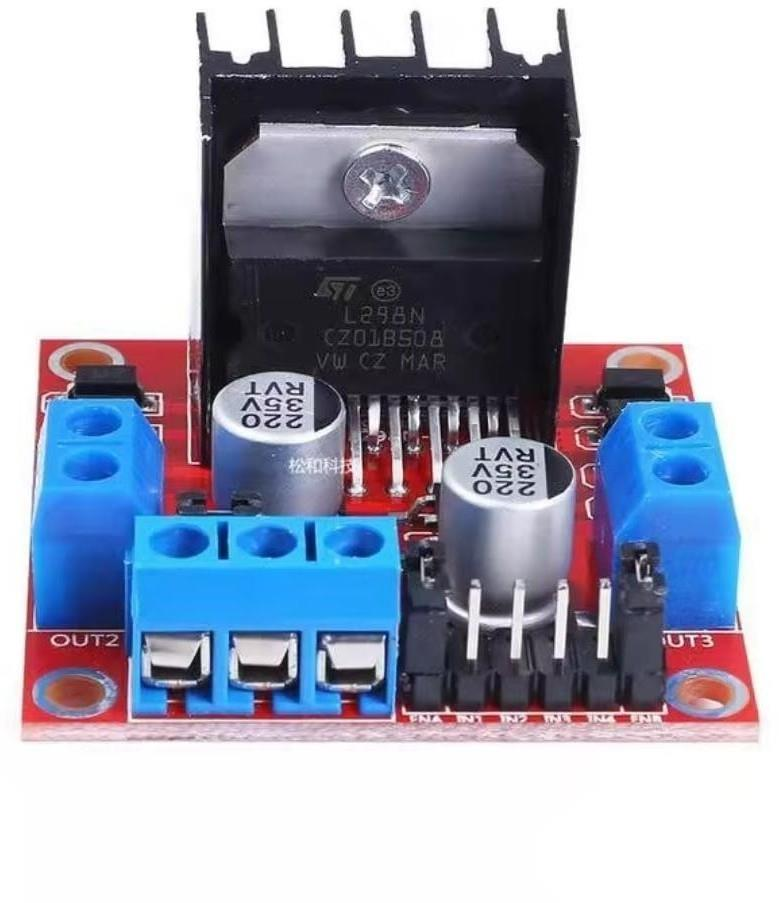
\includegraphics[width=55mm]{figures/fig7_motor_driver.jpg}
\end{center}

\noindent
\begin{spacing}{1.2}
{\fontsize{10.2}{14.5}\selectfont
The motor driver unit used in my project is an L298N motor driver module, which is designed to control the speed and direction of a Permanent Magnet DC (PMDC) motor. It acts as an interface between the microcontroller and the motor because a microcontroller cannot supply the high current required by the motor. The L298N is a dual H-bridge motor driver IC that can control two PMDC motors or one stepper motor. It operates using an external power supply (usually 5V--35V) and provides sufficient current (up to 2A per channel) to drive the motors efficiently.\\[3.5mm]
\textbf{Function:}
\begin{itemize}[leftmargin=8mm, itemsep=2mm, label=\textbullet]
  \item The motor driver works on the H-bridge principle, which allows the motor to rotate in both forward and reverse directions.
  \item When control signals from the microcontroller are applied to the input pins, the driver sends the proper polarity of voltage to the motor terminals.
  \item By changing the logic of the inputs, the direction of current through the motor changes, which changes the rotation direction.
  \item The enable pins control the motor speed using Pulse Width Modulation (PWM) signals.
  \item Thus, the L298N motor driver helps to easily control the speed and direction of a PMDC motor in the project.
\end{itemize}
}
\end{spacing}
\clearpage
